\documentclass{article} 

\usepackage{fancyhdr}
\usepackage[english]{babel}

\usepackage{fullpage}
\usepackage[margin = .75 in]{geometry}
\usepackage[leqno]{amsmath}
\usepackage{amsmath}
\usepackage{amsfonts}
\usepackage{amssymb}
\usepackage{amsthm}
\usepackage{amssymb}
\usepackage[all]{xy}
\usepackage{graphicx}

\usepackage{graphicx,color,url,hyperref}
\usepackage{epsfig}
\fancyhf{}
\setlength{\parindent}{0pt}
\setlength{\parskip}{5pt plus 1pt}
\setlength{\headheight}{13.6pt}

\newcommand{\NN}{\mathbf N}
\newcommand{\RR}{\mathbf R}
\newcommand{\CC}{\mathbf C}
\newcommand{\ZZ}{\mathbf Z}
\newcommand{\ZZn}[1]{\ZZ/{#1}\ZZ}
\newcommand{\QQ}{\mathbf Q}
\newcommand{\nn}{\mathbb N}
\newcommand{\rr}{\mathbb R}
\newcommand{\cc}{\mathbb C}
\newcommand{\zz}{\mathbb Z}
\newcommand{\zzn}[1]{\zz/{#1}\zz}
\newcommand{\qq}{\mathbb Q}
\newcommand{\calM}{\mathcal M}
\newcommand{\latex}{\LaTeX}
\newcommand{\tex}{\TeX}
\newcommand{\dd}{{\rm d}}
\newcommand{\sm}{\setminus} 

\title{Homework 3}
\author{Sunny Lee}
\date{March 30, 2021}

\pagestyle{fancy}
\fancyhf{}
\rhead{March 30, 2021}
\lhead{Sunny Lee}
\chead{Homework 3}
\rfoot{Page \thepage}

\begin{document}

\begin{enumerate}
    \item Let $(V, ||\cdot||)$ be a normed vector space and $x, y\in V$. Then, 
    $||x|| = ||x - y + y|| \leq ||x-y||+||y||$. Since $||x|| \leq ||x-y||+||y||$, 
    $||x|| - ||y|| \leq ||x-y||$. Then, $||x-y|| = ||x + (-y)|| \leq ||x|| + ||-y||
    = ||x|| + |-1|||y|| \leq ||x|| - ||y||$. Since $||x|| - ||y|| \leq ||x-y||$ and
    $||x-y|| \leq ||x|| - ||y||$, $||x-y|| = ||x|| - ||y||$. 

    \item Without loss of generality, let $b > a$. \\
    For Positive Definiteness: \\
    $<f, f>_w = \int_a^bf^2(x)w(x)$. Since $f^2$ is always positive and $w$ is 
    also always positive $f^2(x)w(x)$ is always positive. Since $f^2(x)w(x)$ is 
    always positive and $b > a$, we are going to have a positive value for our 
    integral. \\
    For Symmetry: \\
    $<f, g>_w = \int_a^bf(x)g(x)w(x) = \int_a^bg(x)f(x)w(x) = <g, f>_w$\\
    For Bilinearity: \\
    $<\alpha f+\beta g, h>_w = \int_a^b(\alpha f(x) + \beta g(x))h(x)w(x) = 
    \int_a^b\alpha f(x)h(x)w(x) + \beta g(x)h(x)w(x) = \int_a^b\alpha f(x)h(x)w(x) + \int_a^b\beta g(x)h(x)w(x) =
    <f, h>_w + <g, h>_w$\\
    And thus, since this inner product definition satisfies the properties of an inner
    product, $<f, g>_w = \int_a^bf(x)g(x)w(x)$ is an inner product. 

    \item Let $||x|| = ||y||$. Then, $<x-y, x+y> = (x-y)^T(x+y) = \Sigma (x_i-y_i)(x_i+y_i)
    = \Sigma x_i^2 - y_i^2 = \Sigma x_i^2 - \Sigma y_i^2$. Since $||x|| = ||y||$, 
    $\Sigma x_i^2 - \Sigma y_i^2 = 0$. Thus, $x-y$ is orthogonal to $x+y$ if and only 
    if $||x|| = ||y||$. 

    \item Let $v_0 = 1, v_1 = x, v_2 = x^2, v_3 = x^3$ be the basis vectors given. 
    Then, 
    \begin{gather*}
        y_0 = 1\\
        y_1 = v_1 - <v_1, y_0>\frac{y_0}{||y_0||^2} = x - 0 = x\\
        y_2 = v_2 - <v_2, y_0>\frac{y_0}{||y_0||^2} - <v_2, y_1>\frac{y_1}{||y_1||^2} = x^2 - \frac{1}{3}\\
        y_3 = v_3 - <v_3, y_0>\frac{y_0}{||y_0||^2} - <v_3, y_1>\frac{y_1}{||y_1||^2} - <v_3, y_2>\frac{y_2}{||y_2||^2} = x^3 - \frac{3x}{5}
    \end{gather*}
    Since none of the $y_i$ are zero, we will use all of our $y_i$ in our orthogonal basis. 
    To turn this into an orthonormal basis, we divide each $y_i$ by its inner norm.
    \begin{gather*}
        f_0 = \frac{y_0}{||y_0||} = \frac{1}{\sqrt{2}}\\
        f_1 = \frac{y_1}{||y_1||} = \frac{x}{\sqrt{\frac{2}{3}}}\\
        f_2 = \frac{y_2}{||y_2||} = \frac{x^2 - \frac{1}{3}}{\sqrt{\frac{8}{45}}}\\
        f_3 = \frac{y_3}{||y_3||} = \frac{x^3 - \frac{3x}{5}}{\sqrt{\frac{8}{175}}}
    \end{gather*}
    Since all of the basis vectors are orthogonal, our matrix A will be the 4 by 4
    identity matrix. 

    \item Using Matlab, we can calculate the first 4 terms in our fourier series: \\
    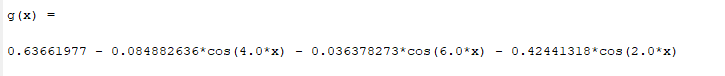
\includegraphics[scale = .9]{5.png}\\
    And thus, our fourier series estimate for $|sin(x)|$ is 
    $0.63661977 - 0.084882636cos(4.0x) - 0.036378273cos(6.0x) - 0.42441318cos(2.0x)$. 
    
    \item Since we are no longer in the interval $[-\pi, \pi]$, we must take back 
    into consideration $L$, our period. We also now have a disctoninuous piecewise 
    function and so when we are integrating, we must split our integral into two 
    parts. Taking this into account, we can write a script in Matlab to get our first
    four fourier series terms: \\
    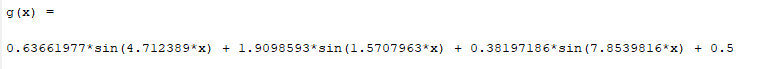
\includegraphics[scale = .9]{6.png}\\
    Plotting these four terms: \\
    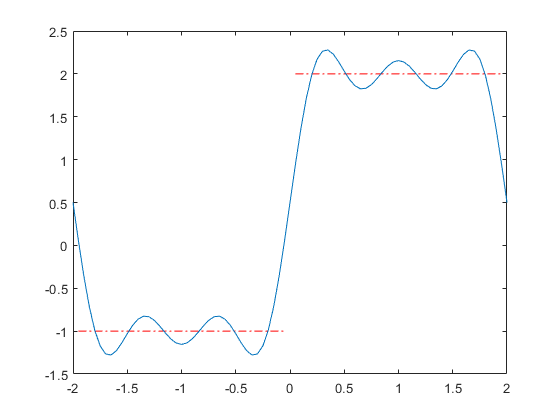
\includegraphics[scale = .7]{6plot.png}

\end{enumerate}

\end{document}